\documentclass[12pt]{article}
 \usepackage[margin=1in]{geometry}
\usepackage{amsmath,amsthm,amssymb,amsfonts}
\usepackage{graphicx}

\newcommand{\N}{\mathbb{N}}
\newcommand{\Z}{\mathbb{Z}}

\newenvironment{question}[2][Question]{\begin{trivlist}
\item[\hskip \labelsep {\bfseries #1}\hskip \labelsep {\bfseries #2.}]}{\end{trivlist}}
%If you want to title your bold things something different just make another thing exactly like this but replace "problem" with the name of the thing you want, like theorem or lemma or whatever

\begin{document}

%\renewcommand{\qedsymbol}{\filledbox}
%Good resources for looking up how to do stuff:
%Binary operators: http://www.access2science.com/latex/Binary.html
%General help: http://en.wikibooks.org/wiki/LaTeX/Mathematics
%Or just google stuff

\title{Week 13}
\author{Kai Lukowiak}
\maketitle
\section{Question}
Use integration by substitution to solve the integral below:
\begin{align*}
\int 4e ^{-7x}dx
\end{align*}
Solved using substitution
\begin{align}
  u=-7x
  \\
  \frac{\partial u}{\partial x} = 7
  \\
  \partial u = (7) \partial x
  \\
  \frac{-4}{7} \int e^u \partial u
  \\
  \frac {-4} {7} e^{-7x} + C
\end{align}

\section{Question}

Biologists are treating a pond contaminated with bacteria. The level of
contamination is changing at a rate of
$\frac {dN} {dt} = \frac {- 3150}{t^4} - 220$ bacteria per cubic centimeter per
day, where t is the number of days since treatment began. Find a function
$N( t )$ to estimate the level of contamination if the level after 1 day was
6530 bacteria per cubic centimetre.

\begin{align}
  \frac {dN} {dt} = \frac {- 3150}{t^4} - 220
  \\
  =
  \\
  \frac {dN} {dt} = -3150 t^{-4}-220
\end{align}
Taking the integral of this we get:

\begin{equation}
  \setcounter{equation}{0}
  \int -3150 t^{-4}-220 \partial t
  \\
  =
\end{equation}

\begin{equation}
  \frac{3150}{3}t^{-3} - 220t +C
\end{equation}

\begin{equation}
  6350 =\frac{3150}{3}1^{-3} - 220 \cdot 1 + C
\end{equation}

\begin{equation}
  C = 6530 + 1270 = 7800
\end{equation}

Therefore the level of contamination is given by:

\begin{equation}
  6350 =\frac{3150}{3}1^{-3} - 220 \cdot 1 + 7800
\end{equation}

\section{Question}
\label{sec:q3}

Find the total area of the red rectangles in the figure below, where the
equation of the line is $f(x)=2x-9$.

\begin{figure}[ht!]
\centering
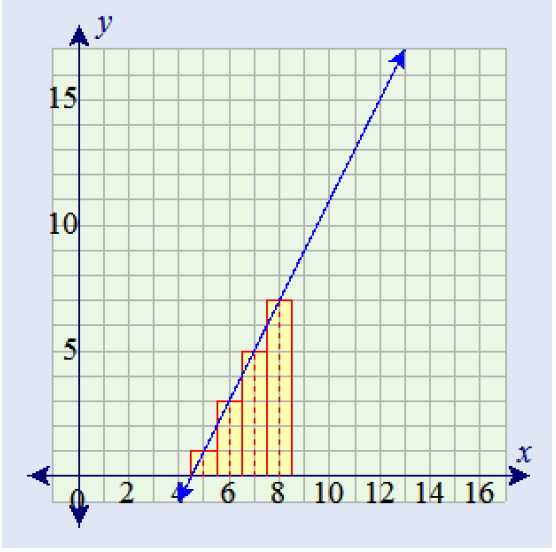
\includegraphics[width=90mm]{graph.png}
\caption{The Graph\label{overflow}}
\end{figure}

The equation for the rectangles is:

\begin{equation}
  \setcounter{equation}{0}
  f(x)=2x-9
\end{equation}
\begin{equation}
  \int_{4.5}^{8.5} 2x-9 dx
\end{equation}

\begin{equation}
  =x^2 - 9x +C
\end{equation}
We can ignore C

\begin{equation}
  [x^2 - 9x]_{4.5}^{8.5}
\end{equation}
\begin{equation}
  8.5^2 - 9 \cdot 8.5 - (4.5^2 - 9 \cdot 4.5)
\end{equation}
\begin{equation}
  = 16
\end{equation}

\section{Question}
\label{sec:q4}

Find the area of the region bounded by the graphs of the given equations.
$y = x^2- 2x- 2, y = x + 2$
\\

Solving the system of equations gives:
\begin{align*}
  x^2-2x-2=x+2
  \\
  x^2-3x - 4 = 0
  \\
  = -1, \quad 4
\end{align*}

Taking the difference between the equations:

\begin{align*}
  x^2-3x - 4
  \\
  \int_{-1}^4 -x^2-3x - 4
  \\
  [\frac{x^3}{3}- \frac{3x^2}{2} - 4x]_{-1}^4
  \\
  \bigg[\frac{64}{3}- \frac{48}{2} - 16 \bigg] - \bigg[\frac{-1}{3}- \frac{3}{2} +4\bigg]
  \\
  =20.83
\end{align*}

\section{Question}
\label{sec:q5}

A beauty supply store expects to sell 110 flat irons during the next year. It
costs \$3.75 to store one flat iron for one year.  There is a fixed cost of
\$8.25 for each order. Find the lot size and the number of orders per year that
will minimize inventory costs.


The let $\alpha$ but the number of irons in an order and $\rho$ be the number of
orders per year. $\alpha \cdot \rho = 110$ which leads to $\alpha = 110/\rho$.d

We assume that the average number of irons at any given time is half the order
size, $\alpha$.

\setcounter{equation}{0}
\begin{align}
  c=8.25 \cdot \rho + \frac{3.75 \alpha}{2}
  \\
  c=8.25 \cdot \rho + \frac{3.75 \cdot 110/\rho}{2}
  \\
  c=8.25 \cdot \rho + \frac{412.5}{2\rho}
  \\
  c=8.25 \cdot \rho + \frac{206.25}{\rho}
  \\
  \frac{\partial c}{\partial \rho} = 8.25 - \frac{206.25}{\rho^2}
\end{align}

To minimize cost we must find the point where $\frac{\partial c}{\partial \rho} = 0$

\begin{align}
  0= 8.25 - \frac{206.25}{\rho^2}
  \\
  8.25 = \frac{206.25}{\rho^2}
  \\
  \rho^2 = \frac{206.25}{8.25}
  \\
  \rho = \sqrt{25}
  \\
  =5
\end{align}

Therefore the company should make five orders of $110/5=22$ irons each.

\section{Question}
\label{sec:q6}

Use integration by parts to solve the integral below:

\begin{align*}
  \int ln(9x)x^6dx
\end{align*}

\setcounter{equation}{0}
\begin{align}
  U= ln9x
  \\
  dU=\frac{1}{x}dx
  \\
  dV=x^6dx
  \\
  V =\frac{x^7}{7}
  \\
  \int UdV = UV - \int VdU
  \\
  ln9x \cdot \frac{x^7}{7} - \frac{1}{7} \int x^7 \cdot \frac{1}{x} dx
  \\
  = ln9x \cdot \frac{x^7}{7} - \frac{1}{7} * \frac{x^7}{7}+c
  \\
  = ln9x \cdot \frac{7x^7}{49} -  \frac{x^7}{49}+c
  \\
  = \frac{x^7}{49}(7 \cdot ln9x - 1) +c
\end{align}


\section{Question}


Determine whether $f(x)$ is a probability density function on the interval
$[1, \quad e^6]$. If not, determine the value of the definite integral:

A probability density function must sum to 1.

\begin{align*}
f(x)=\frac{1}{6x}
\end{align*}


\setcounter{equation}{0}
\begin{align}
  g(x)= \int_{1}^{6e}\frac{1}{6x} dx
  \\
  \frac{1}{6} \int_{1}^{6e}\frac{1}{x} dx
  \\
  \bigg[ \frac{1}{6} lnx \bigg]_1 ^{6e}
  \\
  \bigg[\frac{1}{6} lne^6 \bigg] - \bigg[\frac{1}{6} ln1\bigg]
  \\
  =\frac{1}{6}(6-0)=1
\end{align}

So yes, the function is a probability density function.
\end{document}
%
